
\documentclass[12pt,bezier,amstex]{minimal}
%\usepackage[paperwidth=14in,paperheight=14in,margin=2in,showframe]{geometry}
\paperwidth=55bp%2in = 2x72bp = 144bp
\paperheight=52bp%1.5in = 1.5x72bp = 108bp
\voffset=-15bp
\hoffset=-50bp
%\special{papersize=550bp,270bp}
\usepackage{lipsum}
 % include bezier curves
\renewcommand\baselinestretch{1.0}           % single space
\pagestyle{empty}                            % no headers and page numbers
\oddsidemargin -10 true pt      % Left margin on odd-numbered pages.
\evensidemargin 10 true pt      % Left margin on even-numbered pages.
\marginparwidth 0.75 true in    % Width of marginal notes.
\oddsidemargin  0 true in       % Note that \oddsidemargin=\evensidemargin
\evensidemargin 0 true in
\topmargin -0.75 true in        % Nominal distance from top of page to top of
\textheight 9.5 true in         % Height of text (including footnotes and figures)
\textwidth 6.375 true in        % Width of text line.
\parindent=0pt                  % Do not indent paragraphs
\parskip=0.15 true in
\usepackage{graphicx}
\usepackage{color}		% Need the color package
\usepackage{epsfig}



\begin{document} 
    
%\begin{figure}[htbp]
%\begin{center}

%scalebox{0.5}{\input{eff_err.pdf}}

%\caption{}
%\label{figure:example}
%\end{center}
%\end{figure}
\begin{picture}(0,0)
\put(-18.,-36.5){\scalebox{0.09}{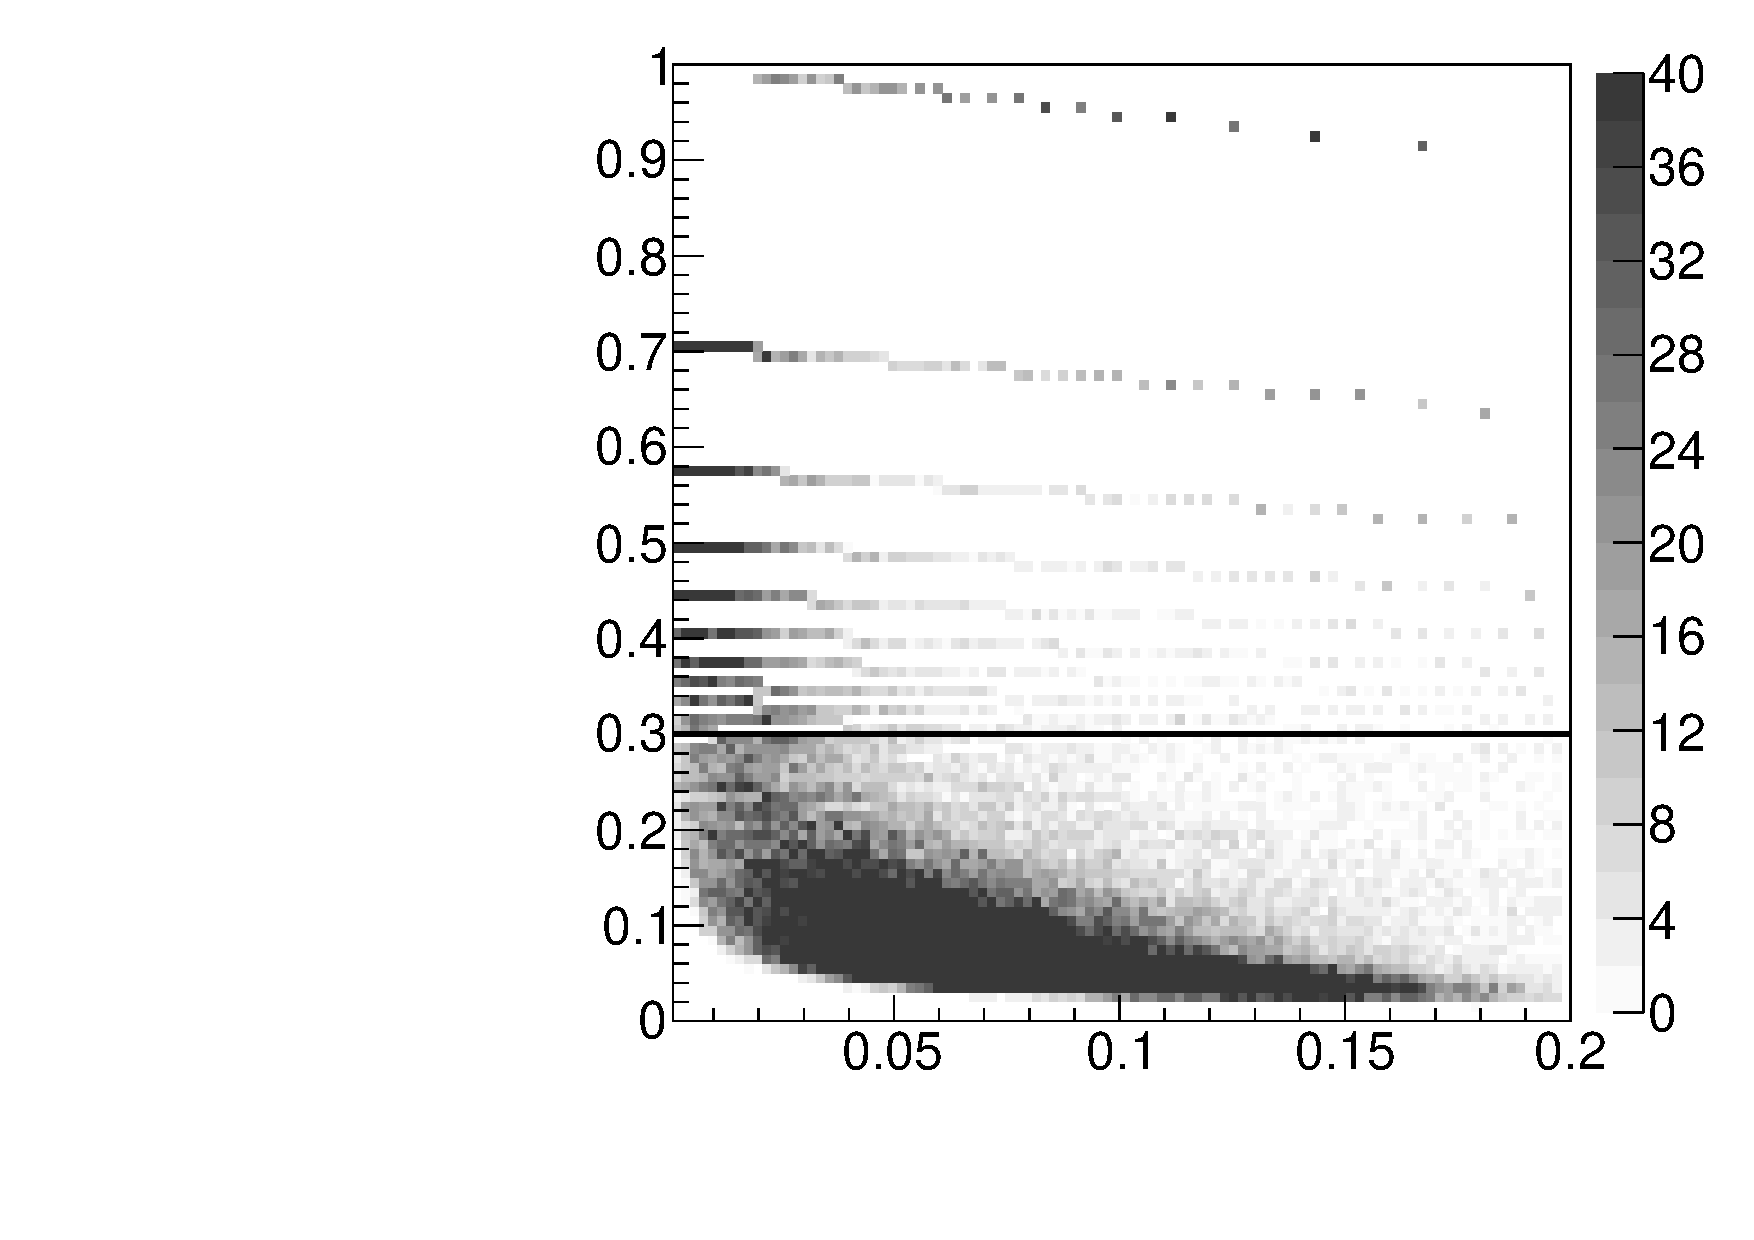
\includegraphics{eff_err.pdf}}}
\put(25.,-36.){\scalebox{0.35}{$\mathcal{E}$}}
\put(-20.,4.){\rotatebox{90.}{\scalebox{0.35}{$\delta\mathcal{E}/\mathcal{E}$}}}

\end{picture}

\end{document}
